% 1.1.Download.tex
%	Last update: 2021/03/02 F.Kanehori
%\newpage
\subsection{ダウンロード}
\label{subsec:Download}
\parindent=0pt

\SprLib はGitHubで管理されており、
次のURLから入手(クローン)することができます。
\begin{center}\Path{https://github.com/sprphys/Springhead}\end{center}

\medskip
\def\tool#1{\hspace{20pt}\makebox[60pt][l]{\tt{#1}}}
\Important{%
	\SprLib のクローン及びビルドには\tt{git}が必要です。
	予めインストールしておいてください。\\
	参考URL:\\
	\tool{git}	  https://gitforwindows.org/\\
	\tool{GUIツール}  https://tortoisegit.org/
}
	
\bigskip
\bf{以下、ダウンロードするディレクトリを\SprTop{}として説明を進めます。}

\bigskip
Explore上で右クリックし``\,Git Clone...\,''を選びます(図\ref{fig:SpringheadClone1})。

Git cloneの画面で、
URLに\tt{https://github.com/sprphys/Springhead}を、
Directoryにダウンロードする場所(この例では\SprTop{})を指定します。
さらにrecursiveにチェックを入れ、OKを押します(図\ref{fig:SpringheadClone2})。
以上で、\SprLib 及びそのサブモジュールがダウンロードされます。

\begin{narrow}[15pt]
	\begin{figure}[h]
	\begin{center}
	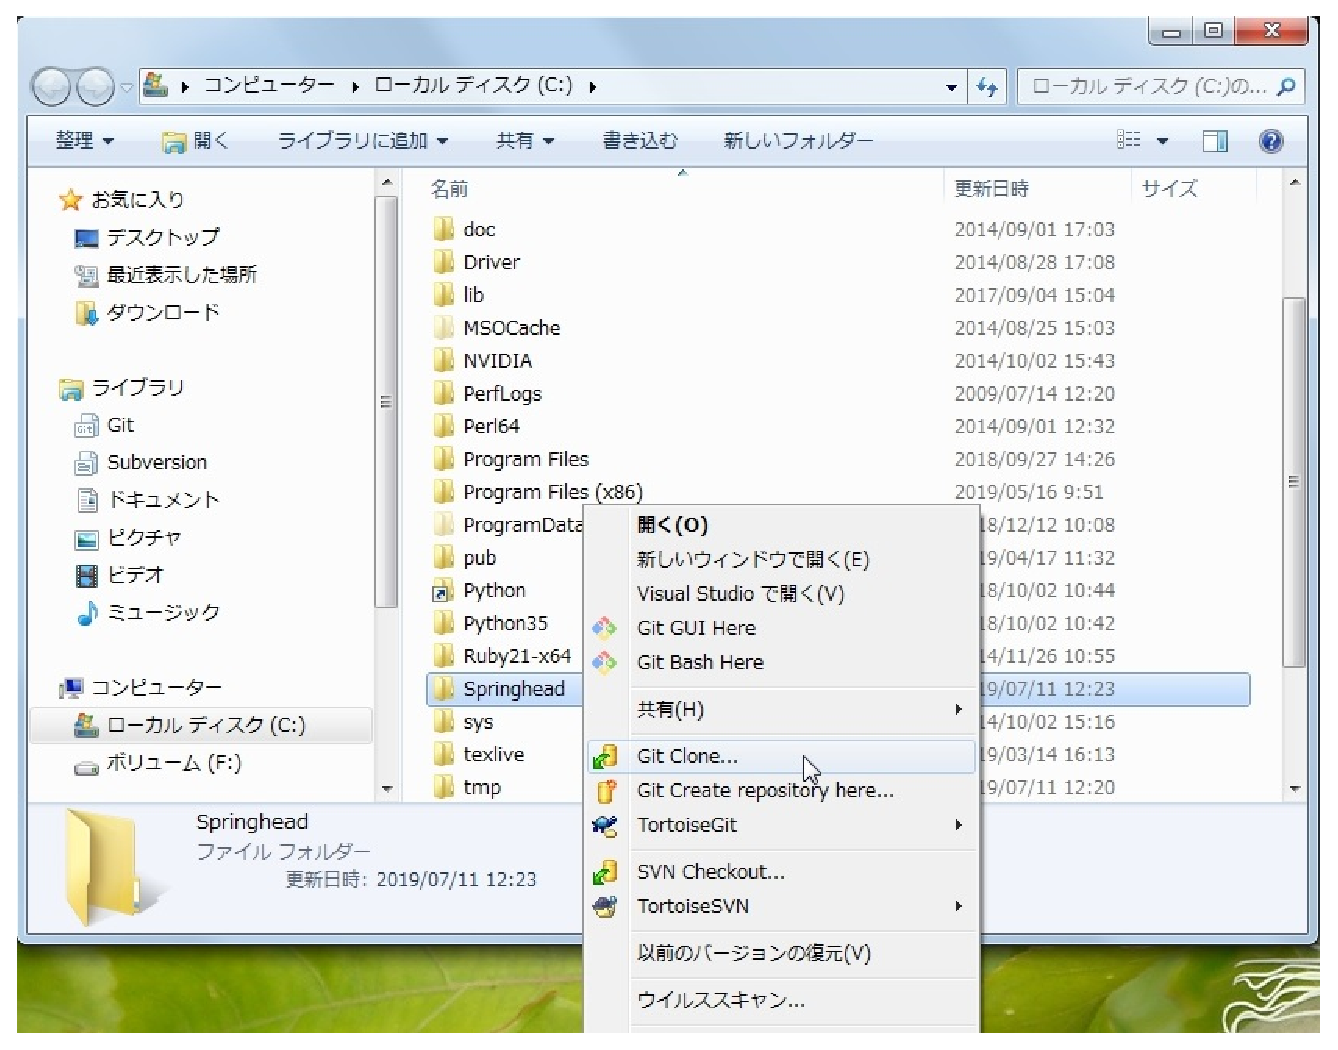
\includegraphics[width=0.5\textwidth]{fig/SpringheadClone1.eps}
	\end{center}
	\caption{Git Clone... の選択}
	\label{fig:SpringheadClone1}
	\end{figure}
\end{narrow}
\begin{narrow}[15pt]
	\begin{figure}[h]
	\begin{center}
	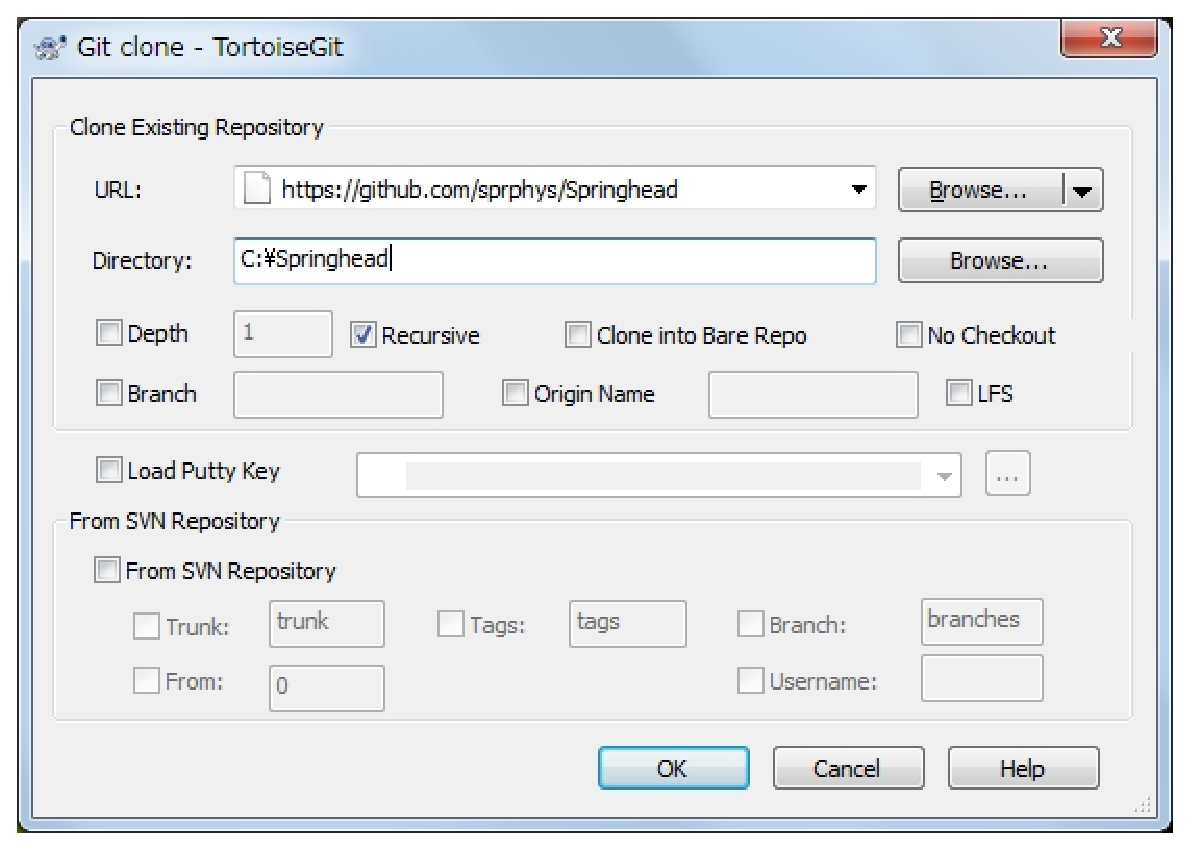
\includegraphics[width=0.5\textwidth]{fig/SpringheadClone2.eps}
	\end{center}
	\caption{URL等の指定}
	\label{fig:SpringheadClone2}
	\end{figure}
\end{narrow}

\medskip
コマンドラインからダウンロードする場合は、次のようにします。

\CmndLine{%
	> chdir C:/Springhead\\
	> git clone --recurse-submodules\Cont\\
	\Hskip{100pt}https://github.com/sprphys/Springhead
}{command-1-1-a.eps}{DownloadTree1}

\bigskip
次に\tt{http://git.haselab.net/haselab/springheadclosed.git}から
closedソースを同様にクローンして\SprTop{\closed}に置きます。

以上でダウンロードは終了です。

\bigskip
% end 1.1.Download.tex
